
%使用XeLaTeX编译
%版权所有,翻版必究
%本文件由程序自动生成,任何修改将被覆盖
%2019 年 01 月 23 日




%\FloatBarrier
\cleardoublepage
\chapter{
模型视图
}\label{c000019}


Qt Widgets中的模型视图非常难用。

在Qt Widgets中的模型视图
架构中,每一个单独的项不是
一个单独的QWidget。
而是通过QPainter进行绘制,
并通过一些函数响应鼠标键盘事件。

这就造成了如果读者想
实现一些复杂的动态效果就
不得不自己实现一个超级复杂
的状态机系统或者将每一个数据项
用诸如QListWidgetItem进行包装,
这样会浪费大量内存。

而在Qt Quick中一切可视元素都是一致的。

视图是QQuickItem的子类,
视图中的每一项也是QQuickItem的子类。
在Qt Quick体系中一切都是对象!

读者可以使用Qt Quick的模型视图架构,
将数据与渲染和控制完全分离。
而且,
这种实现是极其高效的,
即使模型拥有高达数亿元素。
Qt Quick的模型视图架构也可以快速
布局。
最终,只有当前可见部分被渲染,而当前不可见部分
除了布局信息之外,不耗费任何额外资源。




%使用XeLaTeX编译
%版权所有,翻版必究
%本文件由程序自动生成,任何修改将被覆盖
%2019 年 01 月 23 日




%导引

\FloatBarrier
\section{
导引
}\label{c000019s01}


%%%%%%%%%%%%%%%%%%%%%%%%%%%%%%%导引

\FloatBarrier
\subsection{
使用QtCreator快速创建模型
}\label{c000019s01s01}


无论是对于初学者还是老手,
通过继承自QAbstractItemModel
创建自己的模型都是一件麻烦的事。

所幸的是QtCreator可以帮助我们快速的
创建出我们所需的模型的架构。

\begin{enumerate}

\item 如\figurename\ \ref{p000044}所示。
在项目名称单击右键,选择“Add New\ldots”。
\FloatBarrier
%begin图片
\begin{figure}[htb] %浮动体 here and top ...
%there must use marginnote ...
\marginnote{\setlength\fboxsep{2pt}\fbox{\footnotesize{\kaishu\figurename\,}\footnotesize{\ref{p000044}}}}\centering %中心对齐
\setlength\fboxsep{0pt}\fcolorbox[rgb]{0,0,0}{0.97,0.98,0.99}{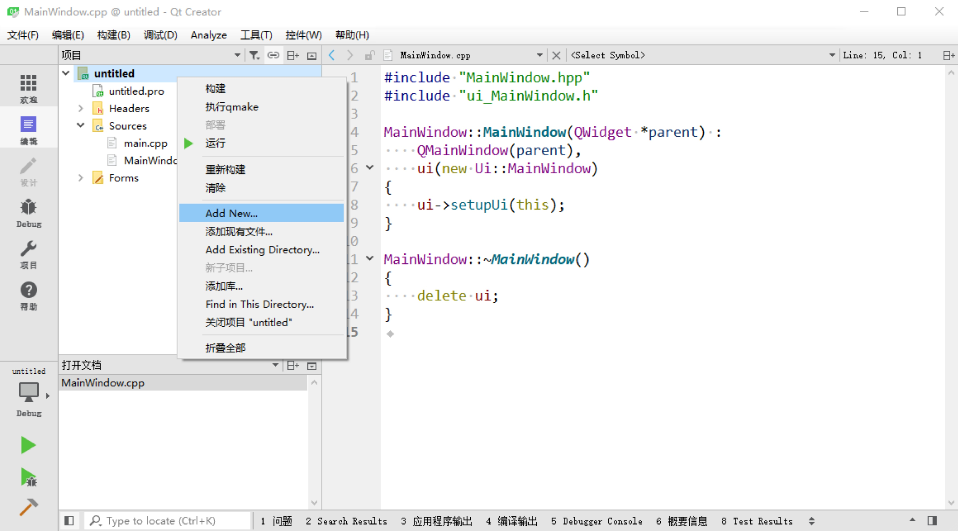
\includegraphics[width=0.95\textwidth]{the_book_image/p000044.pdf}} %图片路径
\caption{使用QtCreator创建模型} %标题
\label{p000044} %索引
\end{figure}
%end图片


\item 如\figurename\ \ref{p000045}所示。
选择“Qt Item Model”模板。
\FloatBarrier
%begin图片
\begin{figure}[htb] %浮动体 here and top ...
%there must use marginnote ...
\marginnote{\setlength\fboxsep{2pt}\fbox{\footnotesize{\kaishu\figurename\,}\footnotesize{\ref{p000045}}}}\centering %中心对齐
\setlength\fboxsep{0pt}\fcolorbox[rgb]{0,0,0}{0.97,0.98,0.99}{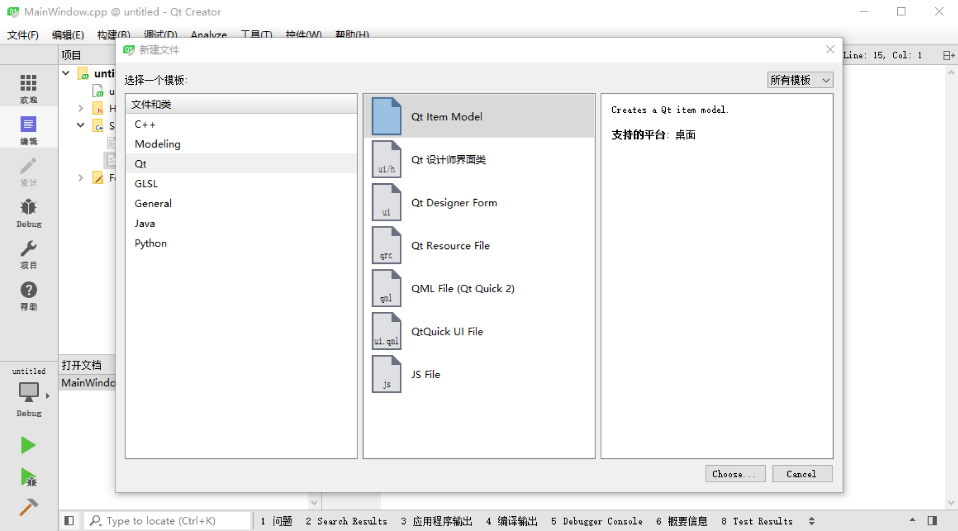
\includegraphics[width=0.95\textwidth]{the_book_image/p000045.pdf}} %图片路径
\caption{使用QtCreator创建模型} %标题
\label{p000045} %索引
\end{figure}
%end图片


\item 如\figurename\ \ref{p000046}所示。
输入类名,并选择所需功能。
如果没有选择任何功能,则创建一个只读的模型。
\begin{tabbing}
\textbullet\ Rows and columns can be removed \hspace{2em} \= MMM \kill
\textbullet\ Customize header row\>
自定义标题 \\
\textbullet\ Items are editable \>
数据元素可编辑 \\
\textbullet\ Rows and columns can be added \>
可以添加行或列 \\
\textbullet\ Rows and columns can be removed \>
可以删除行或列 \\
\textbullet\ Fetch data dynamically \>
下拉获得更多数据  
\end{tabbing}

\FloatBarrier
%begin图片
\begin{figure}[htb] %浮动体 here and top ...
%there must use marginnote ...
\marginnote{\setlength\fboxsep{2pt}\fbox{\footnotesize{\kaishu\figurename\,}\footnotesize{\ref{p000046}}}}\centering %中心对齐
\setlength\fboxsep{0pt}\fcolorbox[rgb]{0,0,0}{0.97,0.98,0.99}{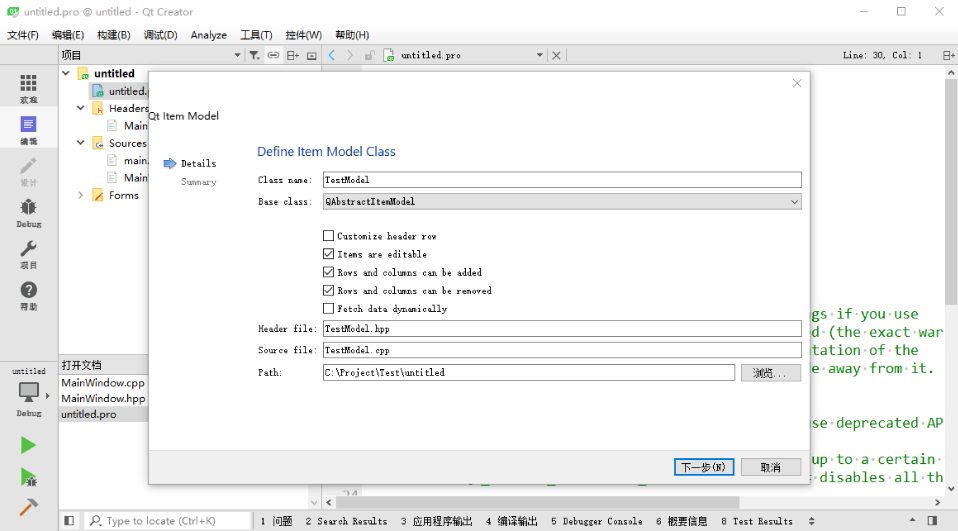
\includegraphics[width=0.95\textwidth]{the_book_image/p000046.pdf}} %图片路径
\caption{使用QtCreator创建模型} %标题
\label{p000046} %索引
\end{figure}
%end图片


\end{enumerate}

%%%%%%%%%%%%%%%%%%%%%%%%%%%%%%%模型与地址
\FloatBarrier
\subsection{
模型与地址
}\label{c000019s01s03}


%begin图片
\begin{figure}[htb] %浮动体 here and top ...
%there must use marginnote ...
\marginnote{\setlength\fboxsep{2pt}\fbox{\footnotesize{\kaishu\figurename\,}\footnotesize{\ref{p000048}}}}\centering %中心对齐
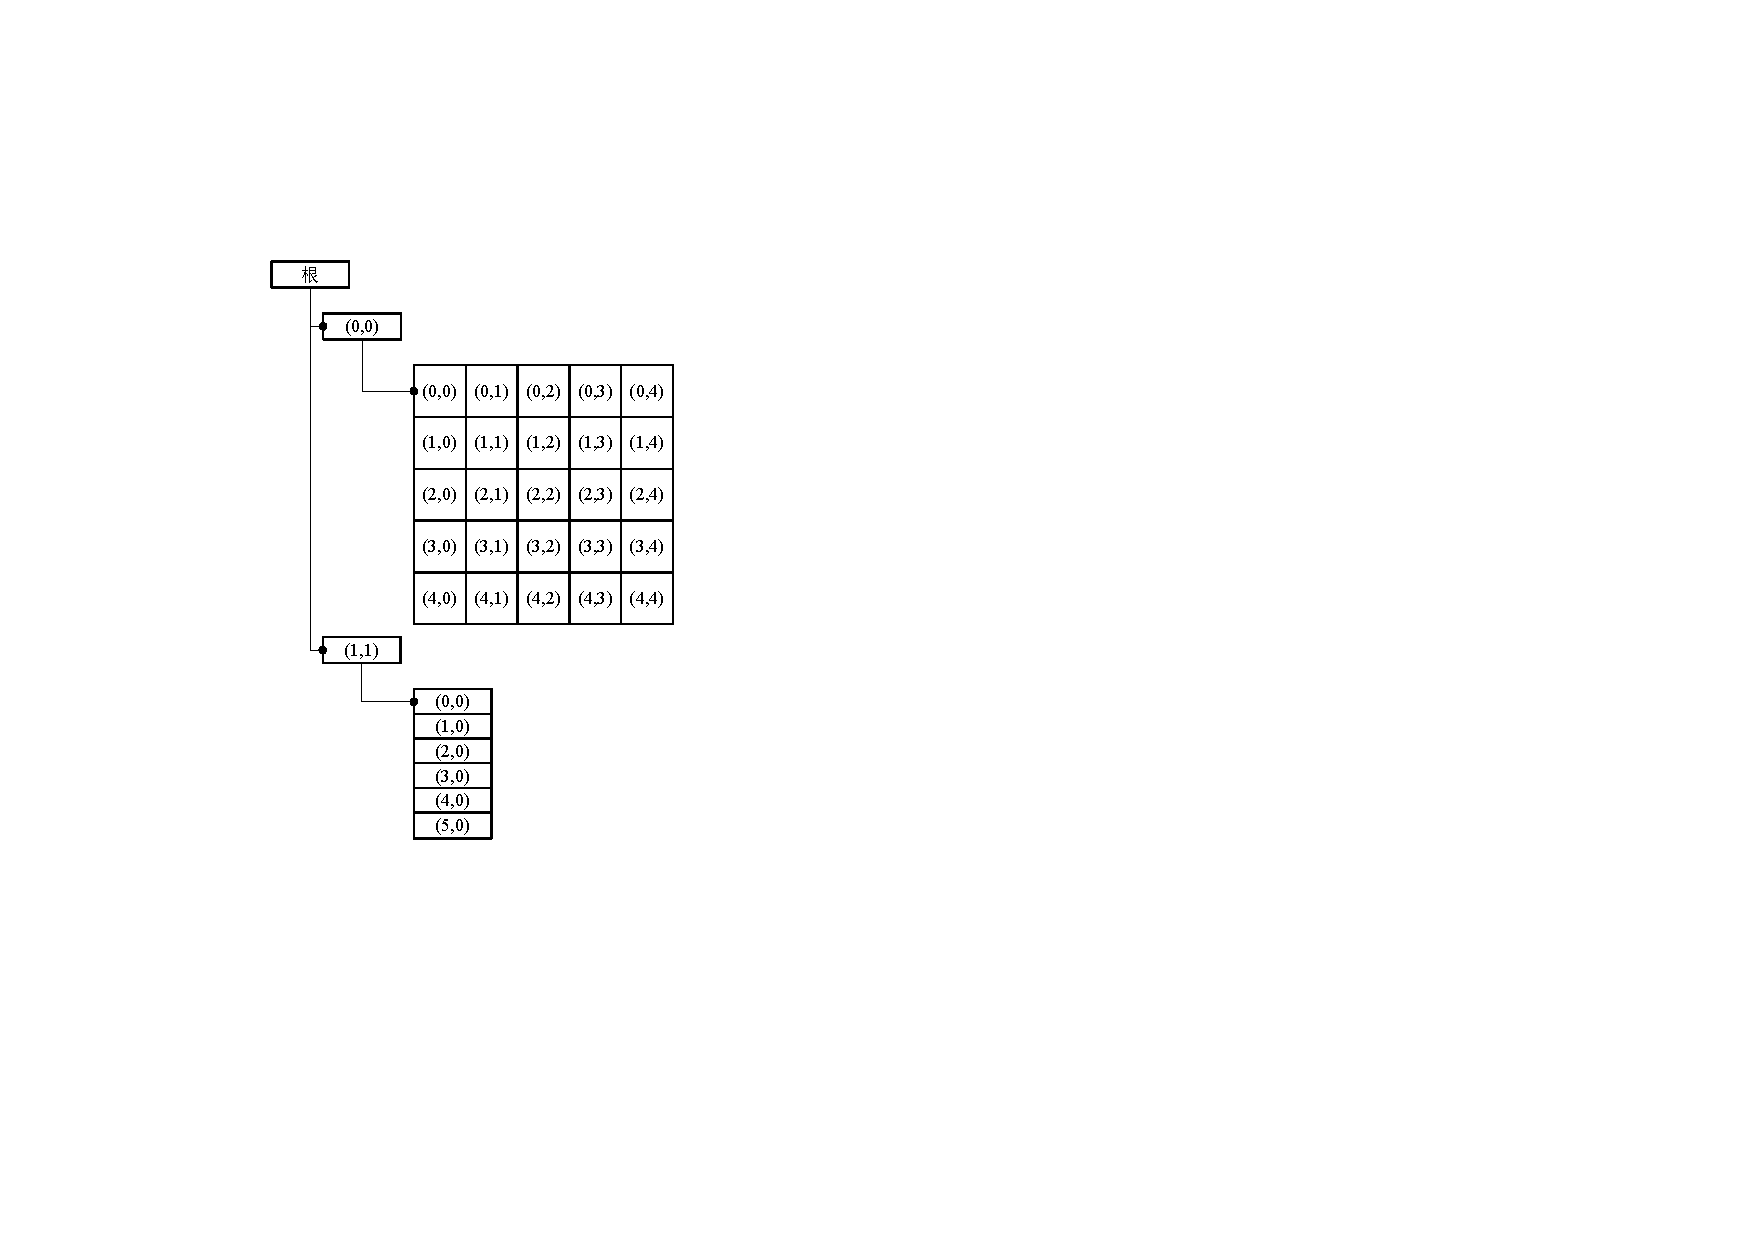
\includegraphics[width=7.5cm]{chapter10/images/ModelAndIndex.pdf} %图片路径
\caption{Qt Model模型} %标题
\label{p000048} %索引
\end{figure}
%end图片


如\figurename\ \ref{p000048},展示了一棵深度
为2的QAbstractItemModel树。

一维表,二维表,树都是通过
QAbstractItemModel
包装的。

%%%%%%%%%%%%%%%%%%%%%%%%%%%%%%%QAbstractItemModel根
\FloatBarrier
\subsubsection{
根
}\label{c000019s01s03s01}

在Qt项视图架构体系里,根是一个无效的QModelIndex。
QModelIndex的默认构造函数就是构造一个无效的索引,也就代表根。

\FloatBarrier
\subsubsection{
项
}\label{c000019s01s03s02}

在Qt项视图架构体系里,项是一个有效的QModelIndex。

一个有效的QModelIndex包含
四个元素:\begin{tabbing}
\hspace*{\parindent}\textbullet\ QAbstractItemModel \raisebox{-0.35ex}{\sourcefonttwo{}*}  \ \ \= \kill
\hspace*{\parindent}\textbullet\ int                   \> row  \\
\hspace*{\parindent}\textbullet\ int                   \> column  \\
\hspace*{\parindent}\textbullet\ quintptr              \> internalid/internalPointer \\
\hspace*{\parindent}\textbullet\ QAbstractItemModel \raisebox{-0.35ex}{\sourcefonttwo{}*}  \> model 
\end{tabbing}
 
一个有效的QModelIndex可以由\begin{littlelongworld}
QModelIndex QAbstractItemModel::createIndex(int r, int c,void \raisebox{-0.35ex}{\sourcefonttwo{}*}p{\sourcefonttwo{}=}nullptr) const
\end{littlelongworld}
或\begin{littlelongworld}
QModelIndex QAbstractItemModel::createIndex(int r, int c,quintptr id) const
\end{littlelongworld}
构造。

QModelIndex与stl迭代器类似,在使用过程中会出现失效问题。
如果需要缓存QModelIndex则需要使用QPersistentModelIndex
进行包装。在使用之前使用\begin{littlelongworld}
bool QPersistentModelIndex::isValid() const
\end{littlelongworld}
进行有效性判断。


\FloatBarrier
\subsubsection{
父项
}\label{c000019s01s03s03}


%%%%%%%%%%%%%%%%%%%%%%%%%%%%%%%QAbstractItemModel重要函数解析
\FloatBarrier
\subsection{
QAbstractItemModel重要函数解析
}\label{c000019s01s02}



\begin{comment}

QHash<int, QByteArray> roleNames() const

Qt::ItemFlags flags(const QModelIndex &index) const

QModelIndex index(int row, int column, const QModelIndex &parent) const
QModelIndex parent(const QModelIndex &index) const

int rowCount(const QModelIndex &parent) const
int columnCount(const QModelIndex &parent) const

QVariant data(const QModelIndex &index, int role) const
bool setData(const QModelIndex &index, const QVariant &value, int role)

bool insertRows(int row, int count, const QModelIndex &parent)
bool insertColumns(int column, int count, const QModelIndex &parent)

bool removeRows(int row, int count, const QModelIndex &parent)
bool removeColumns(int column, int count, const QModelIndex &parent)

\end{comment}




%begin图片
\begin{figure}[htb] %浮动体 here and top ...
%there must use marginnote ...
\marginnote{\setlength\fboxsep{2pt}\fbox{\footnotesize{\kaishu\figurename\,}\footnotesize{\ref{p000047}}}}\centering %中心对齐
\setlength\fboxsep{0pt}\fcolorbox[rgb]{0,0,0}{0.97,0.98,0.99}{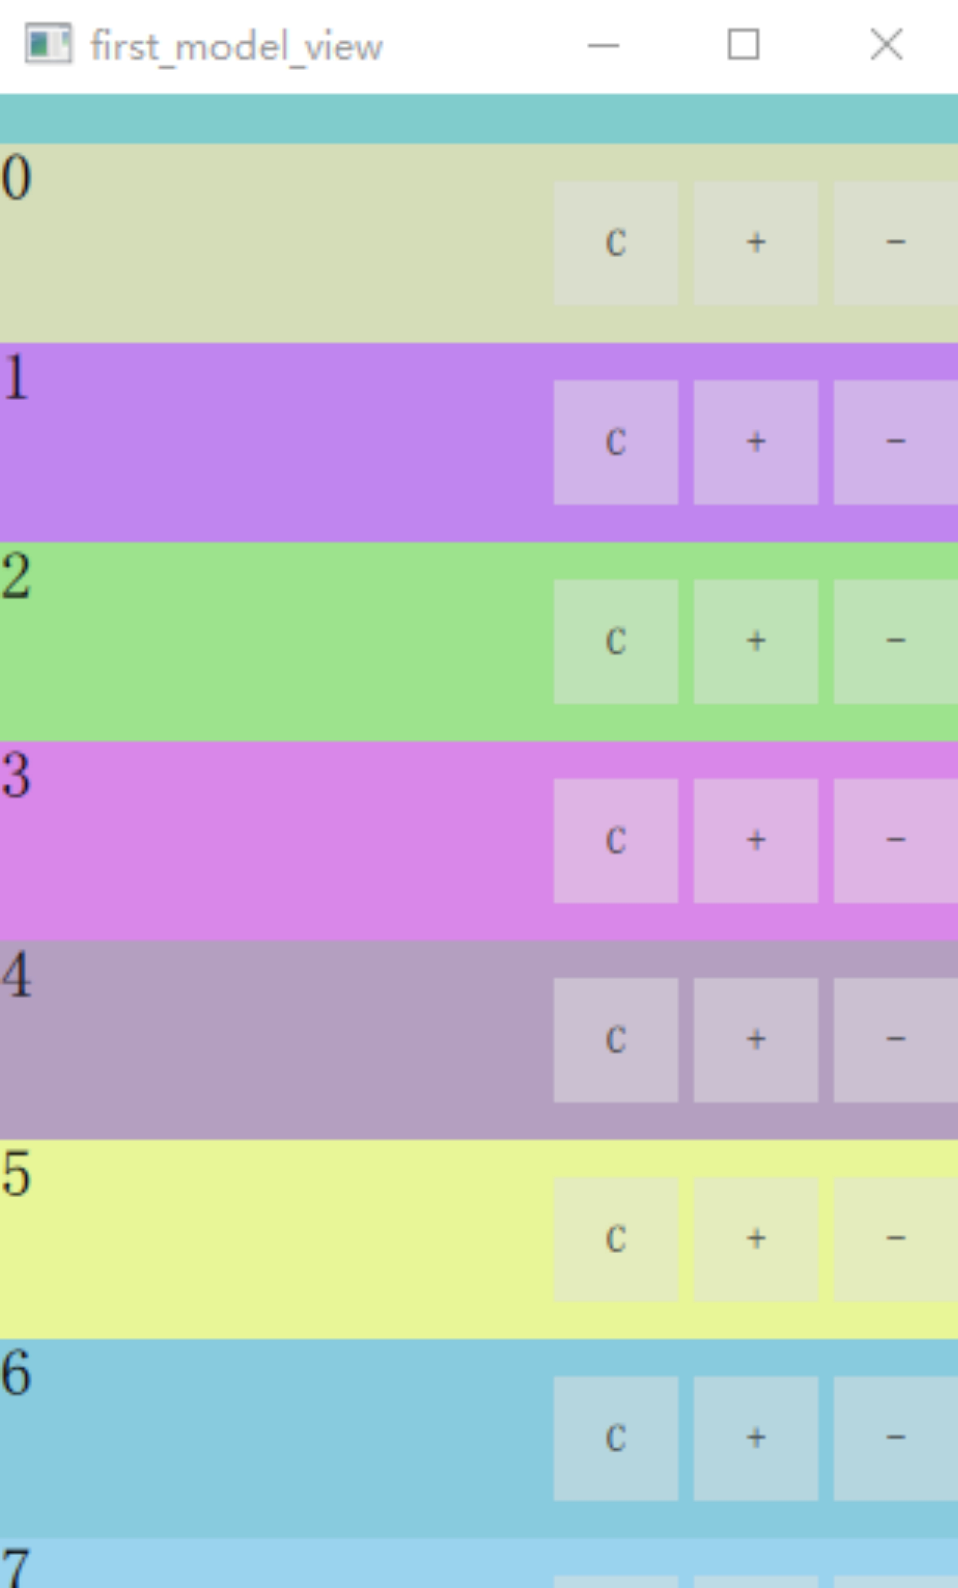
\includegraphics[height=0.75\textwidth]{the_book_image/p000047.pdf}} %图片路径
\caption{List} %标题
\label{p000047} %索引
\end{figure}
%end图片


















%使用XeLaTeX编译
%版权所有,翻版必究
%本文件由程序自动生成,任何修改将被覆盖
%2019 年 01 月 23 日





%使用XeLaTeX编译
%版权所有,翻版必究
%本文件由程序自动生成,任何修改将被覆盖
%2019 年 01 月 23 日




%导引

\FloatBarrier
\section{
自定义树模型
}\label{c000019s02}



% ______all_key_words
% the_book_chapter the_book_subsection the_book_subsubsection
% the_book_section the_book_image the_book_table
% the_book_file the_book_tree_file the_book_command_file
% littlelongworld tabbing ref
% figurename tablename filesourcenumbernameone
% treeindexnumbernameone commandnumbernameone footnote
% item itemize comment textbullet
% \hspace*{\parindent}







%使用XeLaTeX编译
%版权所有,翻版必究
%本文件由程序自动生成,任何修改将被覆盖
%2019 年 01 月 23 日








% ______all_key_words
% the_book_chapter the_book_subsection the_book_subsubsection
% the_book_section the_book_image the_book_table
% the_book_file the_book_tree_file the_book_command_file
% littlelongworld tabbing ref
% figurename tablename filesourcenumbernameone
% treeindexnumbernameone commandnumbernameone footnote
% item itemize comment textbullet
% \hspace*{\parindent}







%使用XeLaTeX编译
%版权所有,翻版必究
%本文件由程序自动生成,任何修改将被覆盖
%2019 年 01 月 23 日



